% ===================================================================
%  Week 1 — Session 2: Images in Code & the Imaging Model
%  Compile: pdflatex -interaction=nonstopmode slides-b.tex  (twice)
% ===================================================================
\documentclass[10pt,aspectratio=169]{beamer}
% ===================================================================
%  Shared Beamer preamble for "Practical Image Processing"
%  English slides. Compile with pdfLaTeX.
% ===================================================================

\usetheme{metropolis}
\usepackage[T1]{fontenc}
\usepackage[utf8]{inputenc}
\usepackage{lmodern}
\usepackage{listings}
\usepackage{tcolorbox}
\usepackage{fontawesome5}
\usepackage{booktabs}
\usepackage{amsmath,amssymb}
\usepackage{tikz}
\usepackage{pgfplots}
\pgfplotsset{compat=1.17}
\usetikzlibrary{arrows.meta,positioning,shapes.geometric,fit,backgrounds,matrix}
\tcbuselibrary{skins,breakable}

% ---- Palette --------------------------------------------------------
\definecolor{coursePrimary}{HTML}{1B4965}   % deep blue
\definecolor{courseAccent}{HTML}{E76F51}    % coral
\definecolor{courseGood}{HTML}{2A9D8F}      % teal
\definecolor{courseBad}{HTML}{C0392B}       % red
\definecolor{courseInfo}{HTML}{2980B9}      % blue
\definecolor{codeBg}{HTML}{F5F6FA}
\definecolor{codeKw}{HTML}{8E44AD}
\definecolor{codeStr}{HTML}{2A9D8F}
\definecolor{codeCom}{HTML}{7F8C8D}

\setbeamercolor{frametitle}{bg=coursePrimary}
\setbeamercolor{progress bar}{fg=courseAccent}
\setbeamercolor{alerted text}{fg=courseAccent}
\metroset{block=fill,sectionpage=progressbar,numbering=fraction}

% ---- Code listings (Python is built into listings) -----------------
\lstdefinestyle{course}{
  backgroundcolor=\color{codeBg},
  basicstyle=\ttfamily\scriptsize,
  keywordstyle=\color{codeKw}\bfseries,
  stringstyle=\color{codeStr},
  commentstyle=\color{codeCom}\itshape,
  numberstyle=\tiny\color{codeCom},
  numbers=left, numbersep=6pt,
  showstringspaces=false, breaklines=true, breakatwhitespace=true,
  tabsize=4, columns=fullflexible,
  frame=single, framesep=4pt, rulecolor=\color{gray!30},
  keepspaces=true, upquote=true, language=Python,
}
\lstset{style=course}
\lstdefinelanguage{bash}{
  keywords={cd,pip,python,venv,source,import}, sensitive=true,
  morecomment=[l]{\#}, morestring=[b]', morestring=[b]",
}

% ---- Reusable callout boxes ----------------------------------------
\newtcolorbox{goodbox}[1][Good practice]{colback=courseGood!8,colframe=courseGood,
  fonttitle=\bfseries,title={\faCheck~#1},boxrule=0.6pt,left=4pt,right=4pt,top=3pt,bottom=3pt}
\newtcolorbox{badbox}[1][Pitfall]{colback=courseBad!8,colframe=courseBad,
  fonttitle=\bfseries,title={\faTimes~#1},boxrule=0.6pt,left=4pt,right=4pt,top=3pt,bottom=3pt}
\newtcolorbox{infobox}[1][Note]{colback=courseInfo!8,colframe=courseInfo,
  fonttitle=\bfseries,title={\faInfoCircle~#1},boxrule=0.6pt,left=4pt,right=4pt,top=3pt,bottom=3pt}
\newtcolorbox{mathbox}[1][Math]{colback=coursePrimary!6,colframe=coursePrimary,
  fonttitle=\bfseries,title={\faCalculator~#1},boxrule=0.6pt,left=4pt,right=4pt,top=3pt,bottom=3pt}

\newcommand{\keyidea}[1]{\begin{alertblock}{Key idea}#1\end{alertblock}}
\newcommand{\term}[1]{\textbf{\color{coursePrimary}#1}}
\newcommand{\code}[1]{\lstinline[basicstyle=\ttfamily\small]|#1|}

% ---- A helper to draw a small pixel grid, cells shaded by value ----
% \pixelgrid{ {10,20,120,200,240}, {30,60,130,180,230}, ... }
\newcommand{\pixelgrid}[1]{%
  \begin{tikzpicture}[font=\scriptsize,scale=0.6]
    \foreach \row [count=\ry] in {#1} {
      \foreach \val [count=\cx] in \row {
        \draw[gray,fill=coursePrimary!8] (\cx,-\ry) rectangle ++(1,-1);
        \node at (\cx+0.5,-\ry-0.5) {\val};
      }
    }
  \end{tikzpicture}}


\title{Digital Images \& the Pipeline}
\subtitle{Week 1 — Session 2: Images in Code \& the Imaging Model}
\author{Practical Image Processing}
\date{Lecture 1.2 \textbullet\ 60--70 min}

\begin{document}

\maketitle

\begin{frame}{Recap of Session 1}
  \begin{columns}[T]
    \begin{column}{0.56\textwidth}
      Last session we established what an image \emph{is}:
      \begin{itemize}
        \item A function $f(x,y)$ \term{sampled} onto a grid and \term{quantized} to integer levels.
        \item Resolution and bit depth set file size and detail.
        \item Color = three numbers per pixel; luminance $\ne$ naive average.
        \item HSV separates color from brightness for robust selection.
      \end{itemize}
    \end{column}
    \begin{column}{0.44\textwidth}
      \begin{infobox}[Today]
        Those numbers, \emph{in code}: NumPy arrays, the \code{uint8} trap, file formats,
        and the physical model that creates every pixel.
      \end{infobox}
    \end{column}
  \end{columns}
\end{frame}

\begin{frame}{The pipeline, again — today's slice}
  \begin{center}
  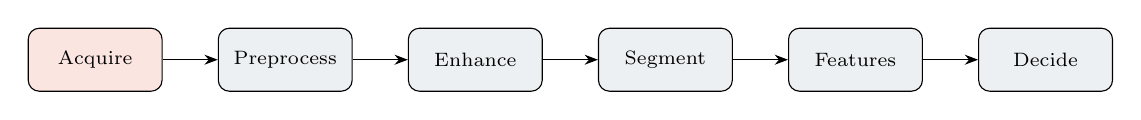
\begin{tikzpicture}[font=\scriptsize,>=Stealth,node distance=3mm and 7mm,
    b/.style={draw,rounded corners,fill=coursePrimary!8,minimum height=8mm,minimum width=17mm,align=center},
    hi/.style={draw,rounded corners,fill=courseAccent!18,minimum height=8mm,minimum width=17mm,align=center}]
    \node[hi] (acq){Acquire};
    \node[b,right=of acq] (pre){Preprocess};
    \node[b,right=of pre] (enh){Enhance};
    \node[b,right=of enh] (seg){Segment};
    \node[b,right=of seg] (feat){Features};
    \node[b,right=of feat] (dec){Decide};
    \draw[->](acq)--(pre);\draw[->](pre)--(enh);\draw[->](enh)--(seg);\draw[->](seg)--(feat);\draw[->](feat)--(dec);
  \end{tikzpicture}
  \end{center}
  \keyidea{Session 2 lives at \term{Acquire}: how pixels enter your program, how they are stored,
  and where their imperfections come from.}
\end{frame}

\begin{frame}{Roadmap}\tableofcontents\end{frame}

% ==================================================================
\section{Images in code}
% ==================================================================

\begin{frame}[fragile]{An image is a NumPy array}
\begin{lstlisting}[language=Python]
import cv2, numpy as np
img = cv2.imread('page.jpg')          # BGR, shape (H, W, 3), dtype uint8
print(img.shape, img.dtype)           # e.g. (1200, 900, 3) uint8
gray = cv2.cvtColor(img, cv2.COLOR_BGR2GRAY)  # (H, W)
print(gray[0, 0])                     # a single pixel's intensity, 0..255
\end{lstlisting}
  \begin{badbox}[OpenCV gotcha]
    OpenCV loads images as \term{BGR}, not RGB. Forgetting this flips red and blue everywhere.
  \end{badbox}
\end{frame}

\begin{frame}[fragile]{Shape and dtype — read them first}
\begin{lstlisting}[language=Python]
print(img.shape)      # (1200, 900, 3)  -> H=1200, W=900, 3 channels
print(img.ndim)       # 3  (color); a grayscale image has ndim == 2
print(img.dtype)      # uint8  -> values 0..255, wraps on overflow
print(img.min(), img.max(), img.mean())   # exposure at a glance
\end{lstlisting}
  \begin{itemize}
    \item \code{shape[0]} is height (rows), \code{shape[1]} is width (columns) — rows come first.
    \item \code{dtype} decides the arithmetic. \code{uint8} is fast and compact but \emph{wraps}.
  \end{itemize}
  \begin{infobox}
    A low \code{mean} = a dark image; a \code{max} well below 255 = never using full brightness.
  \end{infobox}
\end{frame}

\begin{frame}[fragile]{Pixels, slices, and vectorized ops}
\begin{lstlisting}[language=Python]
h, w = gray.shape
roi = gray[100:200, 50:150]           # a rectangular region (a view)
gray[gray < 50] = 0                    # vectorized: threshold dark pixels to black
brighter = np.clip(gray.astype(int) + 40, 0, 255).astype(np.uint8)
\end{lstlisting}
  \begin{goodbox}
    Never loop over pixels in Python — it's 100$\times$ slower. Use NumPy vectorization / OpenCV.
  \end{goodbox}
\end{frame}

\begin{frame}[fragile]{Slicing is $[y, x]$, and a slice is a view}
\begin{lstlisting}[language=Python]
crop = meter[10:38, 60:120]   # rows 10..37, cols 60..119  -> [y, x]!
crop[:] = 0                   # writes THROUGH to `meter` (a view, not a copy)
safe = meter[10:38, 60:120].copy()   # take a copy when you need independence
\end{lstlisting}
  \begin{itemize}
    \item Rows (\(y\)) before columns (\(x\)) — the opposite order of a math point $(x,y)$.
    \item A basic slice shares memory. Mutating it edits the original unless you \code{.copy()}.
  \end{itemize}
  \begin{badbox}
    ``My original changed by itself'' almost always means you mutated a view.
  \end{badbox}
\end{frame}

\begin{frame}[fragile]{Show and save}
\begin{lstlisting}[language=Python]
import matplotlib.pyplot as plt
plt.imshow(cv2.cvtColor(img, cv2.COLOR_BGR2RGB)); plt.axis('off'); plt.show()
cv2.imwrite('gray.png', gray)         # PNG = lossless; JPG would re-compress
\end{lstlisting}
  \begin{infobox}
    Convert BGR$\rightarrow$RGB before \code{plt.imshow}, or your colors look wrong.
  \end{infobox}
\end{frame}

\begin{frame}{The uint8 overflow trap — seen on real data}
  \begin{columns}[T]
    \begin{column}{0.5\textwidth}
      \begin{center}
      
\includegraphics[width=\linewidth]{../assets/meter_bright_ok.png}\\[2pt]
      {\scriptsize \code{+60} done right (clip): uniformly brighter}
      \end{center}
    \end{column}
    \begin{column}{0.5\textwidth}
      \begin{center}
      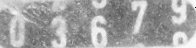
\includegraphics[width=\linewidth]{../assets/meter_bright_overflow.png}\\[2pt]
      {\scriptsize \code{+60} in uint8: bright pixels \emph{wrapped} to dark}
      \end{center}
    \end{column}
  \end{columns}
  \vspace{2pt}
  \begin{badbox}
    $200 + 100 = 44$, not 255. Cast to \code{int}, compute, \code{clip} to 0--255 — or use
    \code{cv2.add} (saturating). A ``brighten'' that darkens bright areas is this bug.
  \end{badbox}
\end{frame}

\begin{frame}{Why $200 + 100 = 44$}
  \begin{mathbox}[The arithmetic behind the trap]
    \code{uint8} holds \(0\)--\(255\): eight bits, \(256\) states. Addition is \emph{modulo} \(256\). \\[3pt]
    \(200 + 100 = 300\), and \(300 \bmod 256 = 300 - 256 = 44.\) \\[3pt]
    The value ``wraps'' past 255 back to 0 and keeps counting — bright turns dark.
  \end{mathbox}
  \begin{itemize}
    \item \code{np.clip(x.astype(int)+100, 0, 255)} promotes to a wide type, then clamps: \(255\).
    \item \code{cv2.add(x, 100)} \term{saturates} in place: anything over 255 sticks at 255.
    \item Same fix, two styles. Both refuse to wrap.
  \end{itemize}
\end{frame}

% ==================================================================
\section{In-class exercise}
% ==================================================================

\begin{frame}[fragile]{\faPen~In-class exercise (10 min)}
  \begin{infobox}[Predict, then run]
    Write your answers down \emph{before} executing the cell.
  \end{infobox}
\begin{lstlisting}[language=Python]
gray = np.array([[100, 150],[200, 250]], dtype=np.uint8)
a = gray + 60          # (1) what are the four values?
b = cv2.add(gray, 60)  # (2) and here?
c = gray.mean()        # (3) what does this represent?
\end{lstlisting}
  \begin{enumerate}
    \item Compute \code{a} by hand — watch the overflow. \quad 2. How does \code{b} differ?
    \item What is \code{c}, and what would a very low \code{c} tell you about the image?
  \end{enumerate}
\end{frame}

\begin{frame}{\faPen~Debrief}
  \begin{itemize}
    \item \code{a} = \code{[[160,210],[4,54]]} — 200+60 and 250+60 \emph{wrapped} (overflow).
    \item \code{b} = \code{[[160,210],[255,255]]} — \code{cv2.add} saturates (clamps to 255).
    \item \code{c} = mean intensity ($\approx$175); a very low mean means a mostly dark image (under-exposed).
  \end{itemize}
  \keyidea{The mean/histogram of an image tells you about exposure before you look at it — Week 2.}
\end{frame}

% ==================================================================
\section{Formats \& storage}
% ==================================================================

\begin{frame}{Image formats: lossless vs lossy}
  \begin{center}
  \begin{tabular}{@{}lll@{}}
    \toprule
    \textbf{Format} & \textbf{Compression} & \textbf{Use} \\
    \midrule
    PNG & lossless & masks, line art, intermediate results \\
    JPEG & lossy & photos; small files, but artifacts \\
    TIFF & lossless/none & archival, scientific, multi-page \\
    BMP/RAW & none & simplicity / sensor data \\
    \bottomrule
  \end{tabular}
  \end{center}
  \keyidea{Never save intermediate results as JPEG — its artifacts corrupt later processing.
  Use PNG until the very end.}
\end{frame}

\begin{frame}{JPEG artifacts matter for processing}
  \begin{itemize}
    \item JPEG discards high-frequency detail in 8$\times$8 blocks — invisible to you, poison to edge detection.
    \item Re-saving a JPEG repeatedly compounds the damage (generation loss).
    \item For DocScan, work from the least-compressed source you can get.
  \end{itemize}
  \begin{infobox}
    A crisp digit edge is exactly the high-frequency content JPEG throws away first —
    the meter and plate crops suffer most where we most need sharpness.
  \end{infobox}
\end{frame}

\begin{frame}{Compression trade-off, in numbers}
  \begin{mathbox}[Worked example]
    A $4000\times3000$ color photo is \(36\) MB uncompressed. Typical stored sizes: \\[3pt]
    \begin{tabular}{@{}lll@{}}
      \toprule
      format & size & ratio \\
      \midrule
      raw / BMP & 36 MB   & 1:1 \\
      PNG (lossless) & \(\sim\)12--20 MB & \(\sim\)2--3:1 \\
      JPEG q=90 & \(\sim\)3--5 MB & \(\sim\)8--12:1 \\
      JPEG q=50 & \(\sim\)1 MB & \(\sim\)36:1 \\
      \bottomrule
    \end{tabular}
  \end{mathbox}
  \begin{itemize}
    \item Lossless buys modest savings for free; lossy buys big savings by \emph{discarding} data.
    \item The savings you cannot see are still gone — decide before, not after, processing.
  \end{itemize}
\end{frame}

\begin{frame}{Bit depth \& dynamic range}
  \begin{itemize}
    \item 8-bit is fine for display; 12--16-bit sensors keep detail in shadows/highlights.
    \item \term{Dynamic range} = ratio of brightest to darkest a sensor can capture.
    \item HDR combines exposures to exceed a single sensor's range (beyond our scope, good to know).
  \end{itemize}
  \begin{infobox}
    Dynamic range is often quoted in \term{stops} (powers of 2): a 12-stop sensor spans a
    \(2^{12} = 4096{:}1\) range from darkest to brightest.
  \end{infobox}
\end{frame}

% ==================================================================
\section{Deep dive: the imaging model}
% ==================================================================

\begin{frame}{Sampling theory \& aliasing}
  \begin{itemize}
    \item \term{Nyquist}: to capture detail at frequency $f$, sample at $>2f$. Under-sample and high frequencies masquerade as low ones.
    \item That's \term{aliasing}: moir\'e patterns, jagged edges, wagon-wheels spinning backwards.
    \item Fix: blur (low-pass) \emph{before} down-sampling — remove detail you can't represent (Week 3, 6).
  \end{itemize}
  \begin{badbox}
    Resizing an image down without blurring first creates aliasing artifacts that no later step can undo.
  \end{badbox}
\end{frame}

\begin{frame}{Aliasing, made concrete}
  \begin{mathbox}[Worked example]
    Suppose the digits on the meter repeat fine texture at \(f = 0.4\) cycles/pixel.
    Nyquist demands a sampling rate above \(2f = 0.8\). \\[3pt]
    Down-sample by 2 (keep every other pixel): the new rate is \(0.5\) — \emph{below} \(0.8\).
    That \(0.4\) texture folds to an alias at \(|0.5 - 0.4| = 0.1\) cycles/pixel: a phantom low-frequency ripple.
  \end{mathbox}
  \begin{itemize}
    \item The fake ripple sits right in the signal band — no later filter can separate it out.
    \item Blur first (kill everything above \(0.25\)), \emph{then} down-sample: nothing is left to fold.
  \end{itemize}
\end{frame}

\begin{frame}{Gamma: pixels aren't linear light}
  \begin{itemize}
    \item Displays and files are \term{gamma-encoded}: pixel value $\ne$ linear light intensity.
    \item Storing perceptually (more codes for dark tones, where eyes are sensitive) saves bits.
    \item For \emph{correct} math (averaging, blending), sometimes linearize first — a common subtle bug.
  \end{itemize}
  \begin{mathbox}
    Encoded $\approx$ (linear)$^{1/\gamma}$, with $\gamma\approx 2.2$. We'll use gamma for contrast in Week 2.
  \end{mathbox}
\end{frame}

\begin{frame}{Gamma, made concrete}
  \begin{mathbox}[Worked example]
    Half the linear light is \emph{not} pixel value \(128\). Encoding \(0.5\) with \(\gamma = 2.2\): \\[3pt]
    \(0.5^{1/2.2} = 0.5^{0.4545} \approx 0.73\), so the stored 8-bit code is \(0.73 \times 255 \approx 186\), not 128. \\[3pt]
    Conversely, code \(128/255 = 0.502\) decodes to \(0.502^{2.2} \approx 0.22\) of full light.
  \end{mathbox}
  \begin{badbox}
    Averaging two gamma-encoded pixels is not the average of their light. For physically
    correct blending, linearize $\rightarrow$ average $\rightarrow$ re-encode.
  \end{badbox}
\end{frame}

\begin{frame}{Where pixels come from}
  \begin{center}
  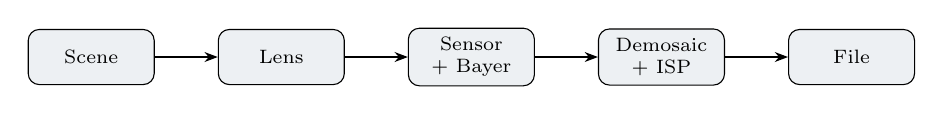
\begin{tikzpicture}[font=\scriptsize,>=Stealth,node distance=3mm and 8mm,
    b/.style={draw,rounded corners,fill=coursePrimary!8,minimum height=7mm,minimum width=16mm,align=center}]
    \node[b] (scene){Scene};
    \node[b,right=of scene] (lens){Lens};
    \node[b,right=of lens] (cfa){Sensor\\+ Bayer};
    \node[b,right=of cfa] (isp){Demosaic\\+ ISP};
    \node[b,right=of isp] (file){File};
    \draw[->](scene)--(lens);\draw[->](lens)--(cfa);\draw[->](cfa)--(isp);\draw[->](isp)--(file);
  \end{tikzpicture}
  \end{center}
  Real sensors capture one color per pixel (a \term{Bayer} mosaic) and interpolate the rest.
  Noise, blur, and color casts enter here — which is exactly what we clean up (Weeks 4, 2).
\end{frame}

\begin{frame}{Noise is physical, not a bug}
  \begin{itemize}
    \item Photon counting is random $\rightarrow$ shot noise; electronics add read noise.
    \item Low light / high ISO = more noise. It's the raw material Week 4 removes.
    \item Understanding \emph{where} noise comes from tells you \emph{how} to model and remove it.
  \end{itemize}
  \begin{infobox}
    Shot noise follows a Poisson law: its standard deviation grows as \(\sqrt{N}\) with the photon
    count \(N\). Brighter pixels are noisier in absolute terms but \emph{cleaner} in relative terms.
  \end{infobox}
\end{frame}

\begin{frame}{Coordinates \& conventions}
  \begin{itemize}
    \item Images are indexed \code{[row, col]} = \code{[y, x]} — the \emph{opposite} of math $(x,y)$.
    \item Origin is top-left; $y$ increases \emph{downward}. This trips up everyone once.
    \item OpenCV points are \code{(x, y)}; NumPy indices are \code{[y, x]}. Keep them straight.
  \end{itemize}
  \begin{badbox}
    Swapping x and y is the \#1 beginner bug in image code. When something's transposed, check this first.
  \end{badbox}
\end{frame}

% ==================================================================
\section{Wrap-up}
% ==================================================================

\begin{frame}{What you should now be able to do}
  \begin{itemize}
    \item Load an image, inspect its shape/dtype, convert color, and slice regions — vectorized.
    \item Explain and avoid the \code{uint8} overflow, BGR-vs-RGB, view-vs-copy, and $x$/$y$ traps.
    \item Choose a format for a task and predict its compression trade-off.
    \item Name where noise, blur, aliasing, gamma, and color casts physically come from.
  \end{itemize}
\end{frame}

\begin{frame}{This week's deliverable}
  \begin{alertblock}{Due before Week 2 (see \code{project/})}
    \begin{enumerate}
      \item Load 3 images; print shape, dtype, min/max/mean; convert to grayscale and to HSV.
      \item Write a correct \code{brighten(img, k)} (no overflow) and compare to \code{cv2.add}.
      \item Take a phone photo of a document — your DocScan test image. Report its properties.
      \item Short note: for your photo, which stages of the pipeline will be hardest, and why?
    \end{enumerate}
  \end{alertblock}
  \begin{goodbox}
    Save every intermediate result as PNG, and print \code{shape}/\code{dtype} at each step — the two habits that prevent most Week 1 bugs.
  \end{goodbox}
\end{frame}

\begin{frame}[standout]
  An image is just numbers on a grid.\\[4pt]
  \normalsize Everything else in this course is arithmetic on those numbers.
\end{frame}

\end{document}
